\PassOptionsToPackage{unicode=true}{hyperref} % options for packages loaded elsewhere
\PassOptionsToPackage{hyphens}{url}
%
\documentclass[]{article}
\usepackage{lmodern}
\usepackage{amssymb,amsmath}
\usepackage{ifxetex,ifluatex}
\usepackage{fixltx2e} % provides \textsubscript
\ifnum 0\ifxetex 1\fi\ifluatex 1\fi=0 % if pdftex
  \usepackage[T1]{fontenc}
  \usepackage[utf8]{inputenc}
  \usepackage{textcomp} % provides euro and other symbols
\else % if luatex or xelatex
  \usepackage{unicode-math}
  \defaultfontfeatures{Ligatures=TeX,Scale=MatchLowercase}
\fi
% use upquote if available, for straight quotes in verbatim environments
\IfFileExists{upquote.sty}{\usepackage{upquote}}{}
% use microtype if available
\IfFileExists{microtype.sty}{%
\usepackage[]{microtype}
\UseMicrotypeSet[protrusion]{basicmath} % disable protrusion for tt fonts
}{}
\IfFileExists{parskip.sty}{%
\usepackage{parskip}
}{% else
\setlength{\parindent}{0pt}
\setlength{\parskip}{6pt plus 2pt minus 1pt}
}
\usepackage{hyperref}
\hypersetup{
            pdfborder={0 0 0},
            breaklinks=true}
\urlstyle{same}  % don't use monospace font for urls
\setlength{\emergencystretch}{3em}  % prevent overfull lines
\providecommand{\tightlist}{%
  \setlength{\itemsep}{0pt}\setlength{\parskip}{0pt}}
\setcounter{secnumdepth}{0}
% Redefines (sub)paragraphs to behave more like sections
\ifx\paragraph\undefined\else
\let\oldparagraph\paragraph
\renewcommand{\paragraph}[1]{\oldparagraph{#1}\mbox{}}
\fi
\ifx\subparagraph\undefined\else
\let\oldsubparagraph\subparagraph
\renewcommand{\subparagraph}[1]{\oldsubparagraph{#1}\mbox{}}
\fi

\usepackage{graphicx}
\usepackage[left=2cm,right=2cm]{geometry}

% set default figure placement to htbp
\makeatletter
\def\fps@figure{htbp}
\makeatother

\newcommand{\mbf}{\mathbf}

\begin{document}

\title{Neuro 120 HW1}
\author{Sam Lurye, Gerardo Parra}
\date{October 4, 2018}
\maketitle

\section*{Problem 1}

\textbf{(a)} See code.
\\\\
\textbf{(b)} When $\Delta t=0.09$, the approximation diverges: the step size is too large, and so our Euler integrator does not effectively approximate the solution to the differential equations, instead returning massive numbers. When $\Delta t=0.07$, the approximation converges; however, the plot of membrane potential is more jagged than when $\Delta t=0.01$.

\section*{Problem 2}

Shortly after the input current is applied, the sodium channel gating variable $m$ begins to increase, so sodium ions begin flowing into the neuron, raising the membrane potential. This in turn causes $m$ to increase even more, beginning a chain reaction, so that the membrane potential jumps rapidly to a peak. Shortly after $m$ begins increasing, $h$ begins to decrease and $n$ begins to increase. The decrease in $h$ corresponds to the inactivation of sodium channels, meaning less sodium flows into the neuron. Meanwhile, the increase in $n$ corresponds to potassium ions flowing out of the neuron. $n$ and $h$ together cause the membrane potential to begin to fall, and as this happens, $m$ begins to decrease, causing the membrane potential to drop even further. Eventually, so much potassium has flowed out of the neuron that the membrane potential is more negative than its resting state. When this happens, $n$ begins to decrease and $h$ begins to increase, so that potassium stops leaving the cell and sodium can begin flowing in again. As a result, the membrane potential is slowly restored to its initial resting state.

\section*{Problem 3}

\textbf{(a) and (b)} The following is a plot of firing rate in Hz versus current in $\mu A$. The minimum sustained firing rate for the HH model is about 53.48 Hz.

\begin{figure}
    \centering
    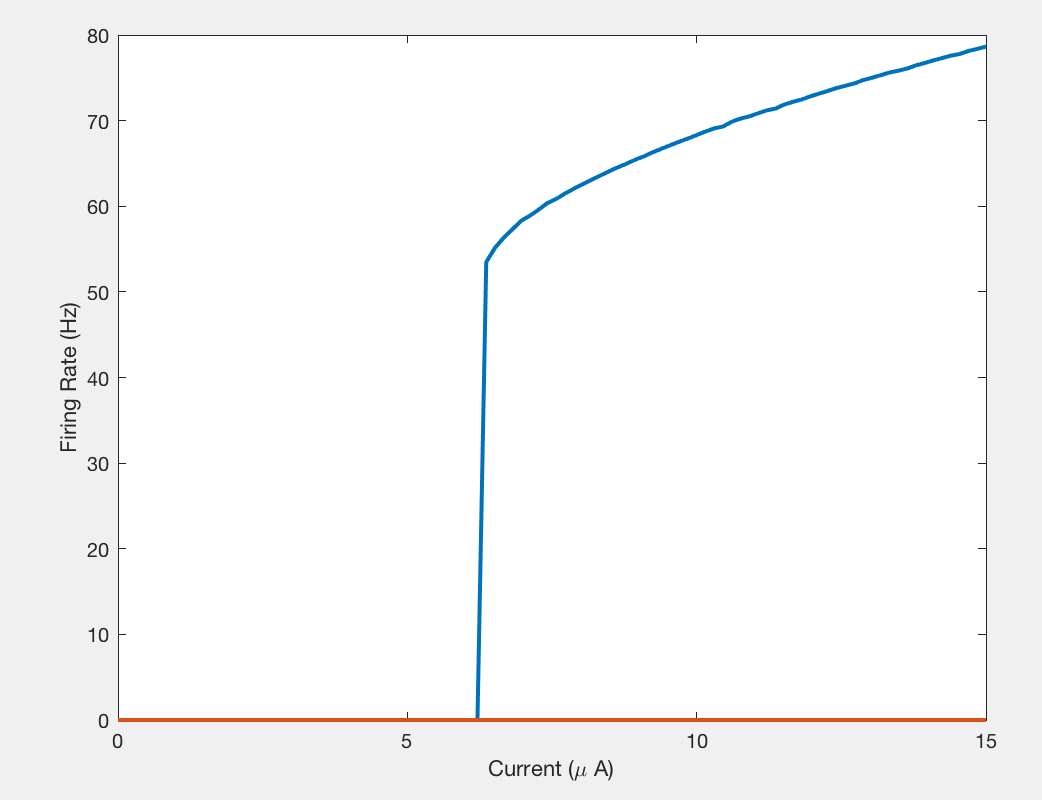
\includegraphics{const_current_firing_rate.png}
    \label{fig:const_current}
\end{figure}

\end{document}
